\documentclass[12pt,letterpaper]{article}
\usepackage{fullpage}
\usepackage[top=2cm, bottom=4.5cm, left=2.5cm, right=2.5cm]{geometry}
\usepackage{amsmath,amsthm,amsfonts,amssymb,amscd}
\usepackage{lastpage}
\usepackage{enumerate}
\usepackage{fancyhdr}
\usepackage{mathrsfs}
\usepackage{xcolor}
\usepackage{graphicx}
\usepackage{listings}
\usepackage{hyperref}



\hypersetup{%
  colorlinks=true,
  linkcolor=blue,
  linkbordercolor={0 0 1}
}

\lstdefinestyle{Python}{
    language        = Python,
    frame           = lines, 
    basicstyle      = \footnotesize,
    keywordstyle    = \color{blue},
    stringstyle     = \color{green},
    commentstyle    = \color{red}\ttfamily
}

\setlength{\parindent}{0.0in}
\setlength{\parskip}{0.05in}

\newcommand\course{CSE 491}
\newcommand\projnumber{2}                  
\newcommand\namea{Gabrielle Talavera}           
\newcommand\nameb{Joshua Hosea}           

\pagestyle{fancyplain}
\headheight 35pt
\lhead{\namea}
\lhead{\namea\\\nameb}                
\chead{\textbf{\Large Project \projnumber}}
\rhead{\course \\ \today}
\lfoot{}
\cfoot{}
\rfoot{\small\thepage}
\headsep 1.5em

\begin{document}

\section*{Nearest Neighbor}
    
    \begin{lstlisting}[style = Python]
    KNN_test(X_train,Y_train,X_test,Y_test,K)
    \end{lstlisting}
    
    \begin{flushleft}To implement this function we had helper functions to compute the distance from the test point to each training points and to predict the label for each Test Data. Once we created those helper functions, we used our helper function to create a numpy array of the predictions for each test point. To find the accuracy we compared the real labels with our predictions. We then counted the amount of times that it was correct and divided that by the total amount of test points.
    \end{flushleft}
    
    
    \begin{lstlisting}[style = Python]
    choose_K(X_train,Y_train,X_val,Y_val)
    \end{lstlisting}
    
    \begin{flushleft}To choose the best K-value we sampled the accuracy through each odd k-value from 1 to the amount of training points. While iterating through we checked that if the old k-value is better than the new k-value, then update it. From there we returned the k-value which had the best accuracy.
    \end{flushleft}
    
    \begin{lstlisting}[style = Python]
    Testing Nearest Neighbor Functions
    \end{lstlisting}
    
    \begin{flushleft}Below you can see the results of the tests using the data provided. It has the classification using different K values, and it also shows the best K value for the data.
    \end{flushleft}
    
    \begin{figure}[htp]
        \centering
        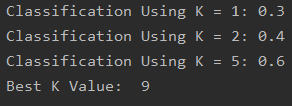
\includegraphics[width=8cm]{knntest.PNG}
        \caption{Nearest Neighbor Function Tests Results}
        \label{fig:knntest}
    \end{figure}
    
\section*{Clustering}
    
    \begin{lstlisting}[style = Python]
    K_Means(X,K)
    \end{lstlisting}
    
    \begin{flushleft}To implement this function we had helper functions to compute the distance from the test point to each training points and to update the cluster centers by finding the average of the distance of the points in each cluster. To actually perform K-Means, we first randomly chose our initial cluster centers using the random function making sure not to choose the same initial cluster. We then keep updating the cluster centers using our helper function until the cluster centers stop changing. From there we return the cluster centers.
    \end{flushleft}
    
    \begin{lstlisting}[style = Python]
    K_Means_better(X,K)
    \end{lstlisting}
    
        \begin{flushleft} For this function we used the data and created a thousand clusters and put that into an array. After putting it into an array we found all the unique cluster center values, and the count of each of those unique values. We used the unique value counts and the values and return the cluster center value that is most frequent from that array. 
    \end{flushleft}
    
    \begin{lstlisting}[style = Python]
    Testing Clustering Functions
    \end{lstlisting}
    
    \begin{figure}[htp]
        \centering
        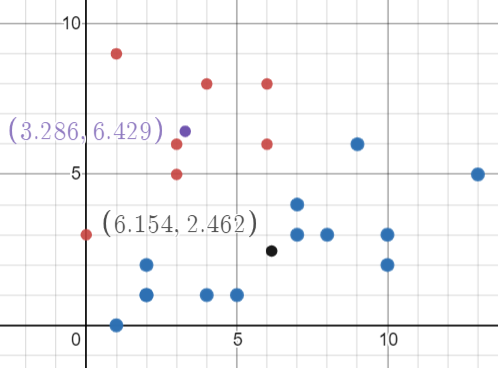
\includegraphics[width=8cm]{cluster2.PNG}
        \caption{Testing K\_Means Where K=2}
        \label{fig:cluster2}
    \end{figure}
    
    \begin{figure}[htp]
        \centering
        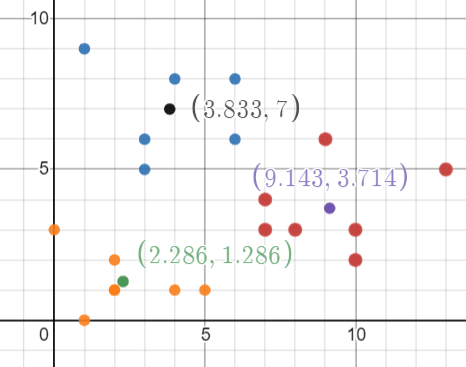
\includegraphics[width=8cm]{cluster3.PNG}
        \caption{Testing K\_Means Where K=3}
        \label{fig:cluster3}
    \end{figure}
    
    \begin{figure}[htp]
        \centering
        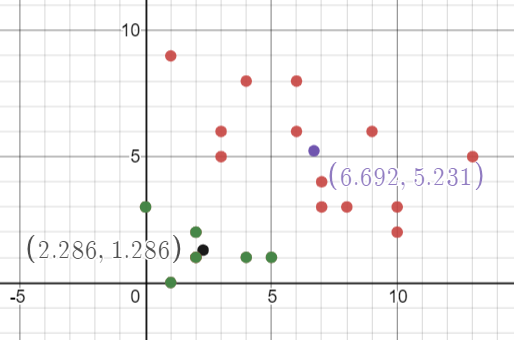
\includegraphics[width=8cm]{bettercluster2.PNG}
        \caption{Testing K\_Means\_Better Where K=2}
        \label{fig:bettercluster2}
    \end{figure}

    \begin{figure}[htp]
        \centering
        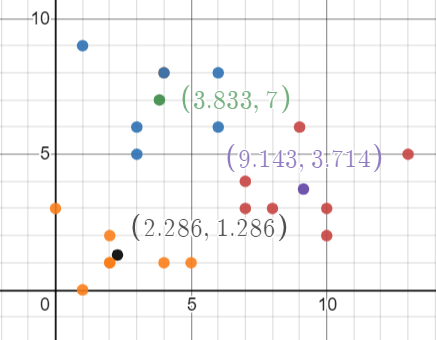
\includegraphics[width=8cm]{bettercluster3.PNG}
        \caption{Testing K\_Means\_Better Where K=3}
        \label{fig:bettercluster3}
    \end{figure}
    

\section*{Perceptron}
    
    \begin{lstlisting}[style = Python]
    perceptron_train(X,Y)
    \end{lstlisting}
    
    \begin{flushleft}For this function we had a helper function to update the weights and bias. We started the weights and bias at 0 and go through one epoch at a time until the previous weights and bias is equal to the current weights and bias. We had a boolean to keep track of whether the weights and bias have been updated on the most current epoch. We would go through each sample in the iteration and update it if the activation was less than or equal to zero. The function returned the weights and bias after all the updating.
    \end{flushleft}
    
    \begin{lstlisting}[style = Python]
    perceptron_test(X_test, Y_test, w, b)
    \end{lstlisting}
    
    \begin{flushleft}For this function we had a count which kept track of how many labels that were correct. To get the number of correct labels we iterated through all the testing samples and calculated the activation for each sample. If the activation multiplied by the label was positive, then we incremented the count. To get the accuracy we got the count of the correct labels divided by the number of samples.
    \end{flushleft}
    
    \begin{lstlisting}[style = Python]
    Training a Perceptron
    \end{lstlisting}
    
    \begin{flushleft}When training the perceptron, we got weights of 2 and 4 and the bias as 2. The image below shows the plot of our decision boundary using the weights and biases we found from the data provided.
    \end{flushleft}

    \begin{figure}[htp]
        \centering
        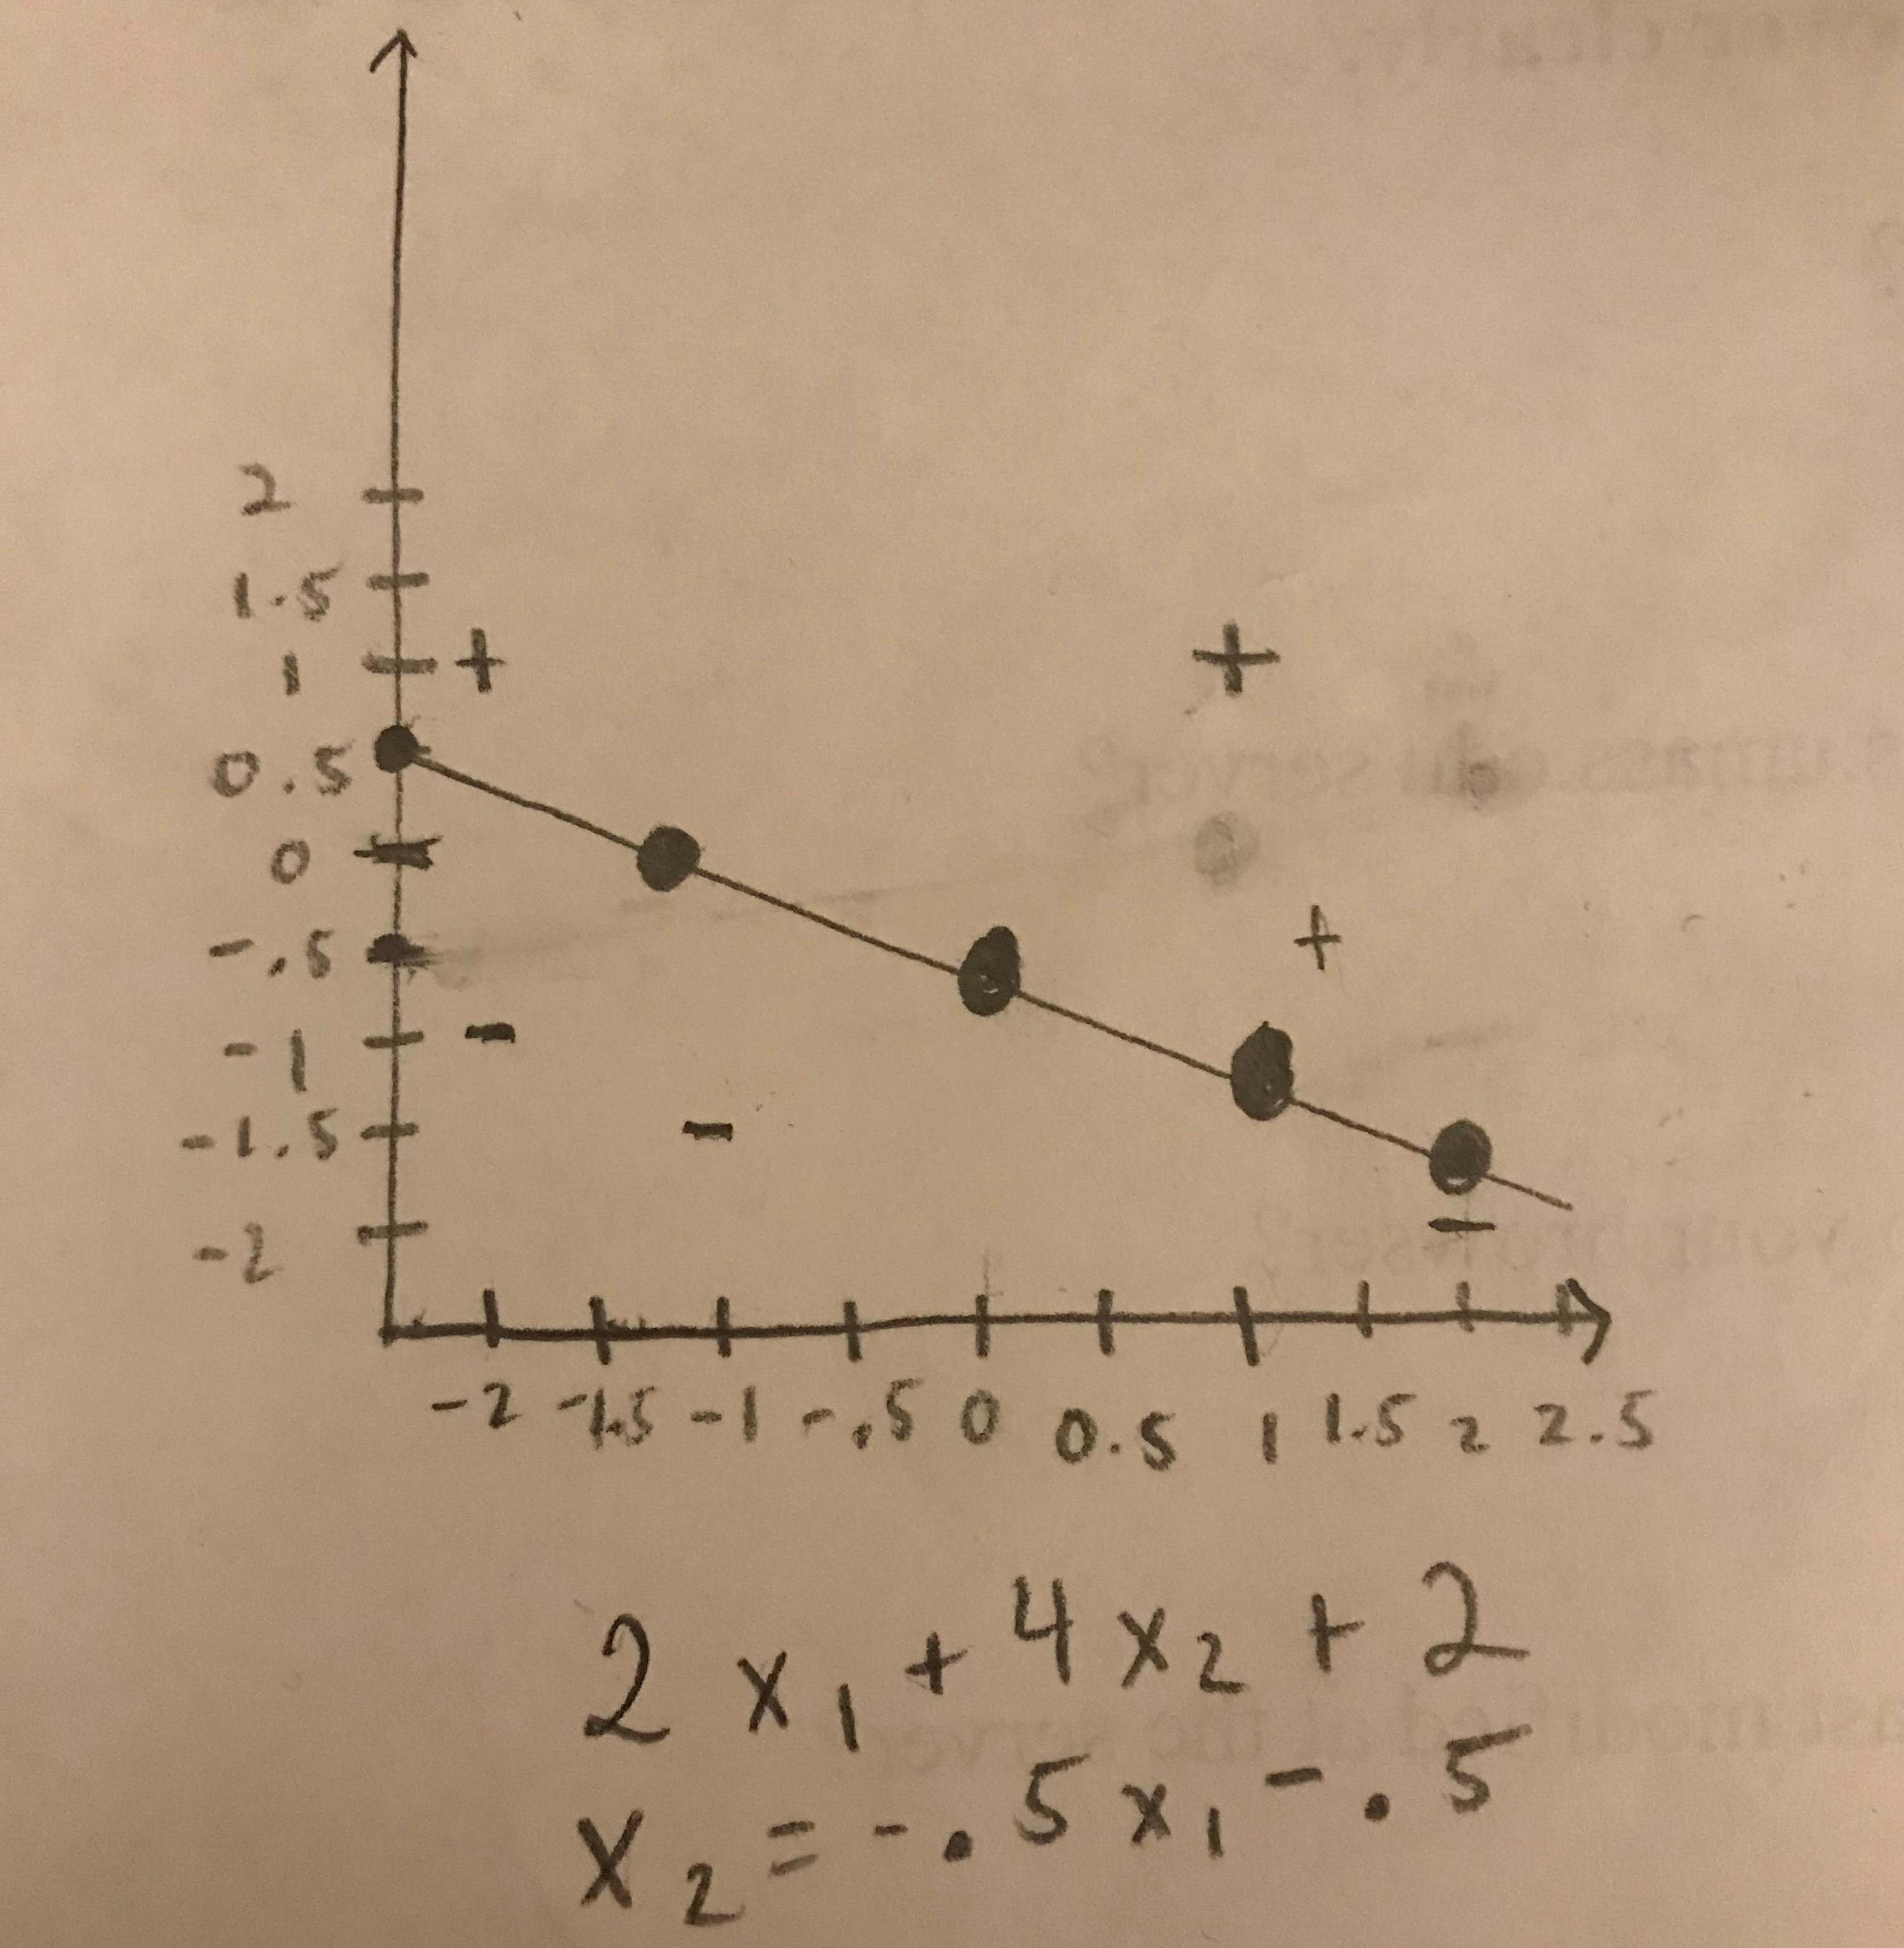
\includegraphics[width=4cm]{decisionboundary.jpg}
        \caption{Perceptron Decision Boundary Plot}
        \label{fig:decisionboundary}
    \end{figure}
    
\end{document}
